% ----------------------------------------------------------
% Teste test5_3_e50b128class10_20231212_034108
% ----------------------------------------------------------
\subsubsection{Teste test5_3_e50b128class10_20231212_034108 - AlexNet (Is That a Santa)}

Informações utilizadas para o treinamento.

\begin{table}[ht]
   \centering
   \caption{Treinamento}
   \label{tab:modelos}
   \begin{tabular}{| c | c | }
      \hline 
      \textbf{Informação} & \textbf{Descrição} \\
      \hline \hline 
      Rede & AlexNet \\
      \hline
      Número de épocas & 50\\
      \hline
      Tamanho do lote & 128\\
      \hline
      Taxa inicial & 0.01 \\
      \hline
      Taxa de decaimento & 0.0005 \\
      \hline
      Total de classes & 10\\
      \hline
      Dataset & CIFAR-10\\
      \hline
   \end{tabular} 
\end{table}

Resultados obtidos após treinamento.

\begin{tabular}{lrrrr}
\toprule
  Unnamed: 0 &  precision &  recall &  f1-score &    support \\
\midrule
    airplane &   0.869180 &  0.7840 &  0.824395 &  1000.0000 \\
  automobile &   0.919171 &  0.8870 &  0.902799 &  1000.0000 \\
        bird &   0.726708 &  0.7020 &  0.714140 &  1000.0000 \\
         cat &   0.699625 &  0.5590 &  0.621456 &  1000.0000 \\
        deer &   0.647232 &  0.8770 &  0.744798 &  1000.0000 \\
         dog &   0.781038 &  0.6920 &  0.733828 &  1000.0000 \\
        frog &   0.799078 &  0.8670 &  0.831655 &  1000.0000 \\
       horse &   0.785649 &  0.8650 &  0.823417 &  1000.0000 \\
        ship &   0.900000 &  0.8730 &  0.886294 &  1000.0000 \\
       truck &   0.888774 &  0.8630 &  0.875698 &  1000.0000 \\
    accuracy &   0.796900 &  0.7969 &  0.796900 &     0.7969 \\
   macro avg &   0.801646 &  0.7969 &  0.795848 & 10000.0000 \\
weighted avg &   0.801646 &  0.7969 &  0.795848 & 10000.0000 \\
\bottomrule
\end{tabular}


\begin{figure}[ht]
 \begin{center}
   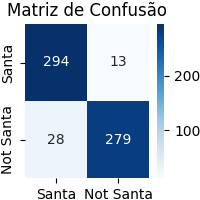
\includegraphics[scale=1]{tests/test5_3_e50b128class10_20231212_034108/confusion_matrix.png}
  \caption{Matriz de Confusão}
  \label{fig:fig03}
 \end{center}
\end{figure}

\begin{figure}[ht]
 \begin{center}
   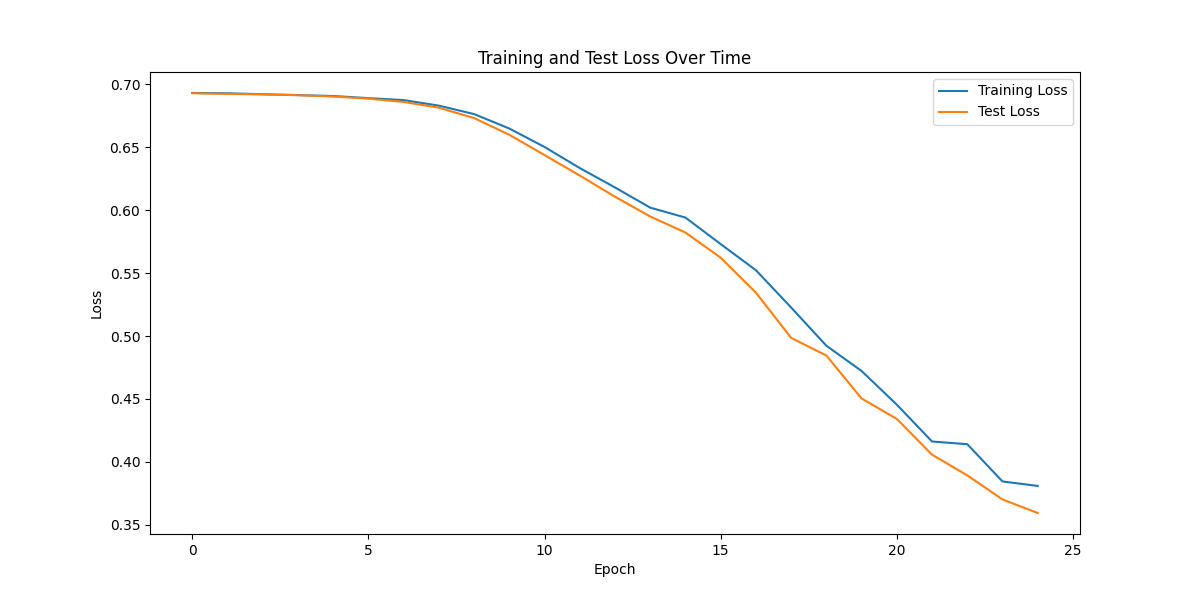
\includegraphics[scale=0.8]{tests/test5_3_e50b128class10_20231212_034108/loss_over_time.png}
  \caption{Gráfico de Perda}
  \label{fig:fig04}
 \end{center}
\end{figure}
